\section{I курс}

\AddProb Два тела бросили одновременно из одной точки: одно вертикально вверх, другое под углом $\varphi~=~30^{\circ}$ к горизонту. 
Начальная скорость каждого тела $v$~=~10 м/с. Найти расстояние между телами через $t$~=~1~с.

\AddProb Тонкий стержень массы $m$ и длины $l$ лежит на гладкой горизонтальной поверхности. Пластилиновый шарик массы $m$ со скоростью $v$, 
перпендикулярной к стрежню, ударяется об один из его концов и прилипает к нему. Какое количество теплоты выделится при таком ударе?

\begin{wrapfigure}{r}{3cm}
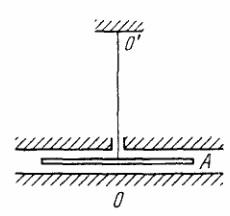
\includegraphics[scale=0.5]{1309OscillationsDisc.jpg}
\end{wrapfigure}

% Почти задача (179) Колебания
\AddProb Тонкий однородный диск массы $m$ и радиуса $R$, подвешенный в горизонтальном положении к упругой нити, совершает крутильные колебания в жидкости. 
Момент упругих сил со стороны нити $M~=~\alpha\,\varphi$.  Сила сопротивления на единицу поверхности $F~=~\beta\,v$, где $v$ -- локальная скорость 
движения диска. Найти частоту малых колебаний.


\section{II и III курсы}

\AddProb Магнитная лента с катушки протягивается через звукосниматель с постоянной скоростью $v$. Толщина ленты равна $h$. 
Найти угловую скорость катушки как функцию времени $t$, если в момент времени $t$~=~0 радиус внешнего слоя магнитной ленты равен $R$.

\AddProb С какой силой давит на землю кобра, когда она, готовясь к прыжку, поднимается вертикально вверх с постоянной скоростью $v$? 
Масса змеи $m$, ее длина $l$.

\AddProb Катушка состоит из среднего цилиндра радиусом $r$ и двух крайних цилиндров радиусами $R > r$. Длинный тонкий провод плотно наматывают на катушку 
следующим образом: сначала обматывают один из крайних цилиндров, а затем продолжают наматывать этот же провод на средний цилиндр в том же 
направлении, в каком начинали намотку. После завершения намотки катушку кладут на горизонтальный стол, помещённый в однородное постоянное магнитное поле $B$, 
линии индукции которого параллельны оси катушки. К первому концу провода, лежащему на столе, подсоединяют идеальный вольтметр, а другой конец провода, 
касающийся неподвижного скользящего контакта, соединённого с вольтметром, начинают тянуть вдоль поверхности стола с постоянной скоростью $v$ в направлении, 
перпендикулярном оси катушки. Считая, что катушка катится по столу без проскальзывания, найдите показания вольтметра.